\documentclass{beamer}
\usetheme{Madrid}

\usepackage{pgfplots}

\usepackage{bm}

\usepackage{graphicx}
\graphicspath{ {img/} }

\title{Stochastic Gradient Descent}
\subtitle{STAT 672 Project}
\author{Tom Wallace}
\institute{George Mason University}
\date{Spring 2018}


\begin{document}

\frame{\titlepage}

%%%%%%%%%%%%% Introduction %%%%%%%%%%%%%%

\begin{frame}
	\frametitle{Optimization is everywhere, and sometimes is easy}
	Many statistical procedures involve minimizing or maximizing some function 
	applied to data \\~\\

	In \textbf{parametric} statistics, we often make assumptions that make this optimization ``nice'':
	\begin{itemize}
		\item \small Example: in OLS, we do not need to check every possible value
			of $\hat{\beta}$ to see if it minimizes the loss
			function, we (typically) can just evaluate
			$(X'X)^{-1}X'Y$ \\~\\
	\end{itemize}
	\smallskip

	\centering
	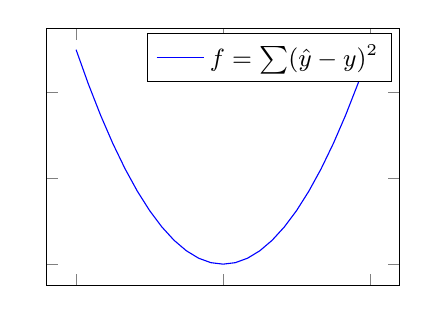
\begin{tikzpicture}
		\begin{axis}[
			yticklabels={,,},
			xticklabels={,,},
			width=0.5\textwidth,
			height=0.4\textwidth,
			legend style = {font=\small}
		]
			\addlegendentry{$f=\sum (\hat{y} - y)^2$}
			\addplot[mark=none, color=blue]{x^2};
		\end{axis}
	\end{tikzpicture}
\end{frame}

\begin{frame}
	\frametitle{Other times, optimization is not so easy}
	Suppose that we have a typical supervised classification problem:
	\begin{itemize}
		\item \small Non-parametric: no assumptions about distribution of data
		\item Feature vector $\mathbf{X}_i$, label $Y_i$
		\item Want to find best prediction function $f^*$ from class $\mathcal{F}$
		\item $f$ has parameter vector $\bm{\theta}$
		\item Optimization: pick values for $\bm{\theta}$ that minimize
			empirical risk according to some
			loss function $L$
		\item Assume $L$ is convex (if not, problem is \textit{much}
			harder)\\~\\
	\end{itemize}

	Our lack of assumptions requires a different approach to optimization
	\begin{itemize}
		\item \small Cannot analytically identify stationary point
		\item Need to numerically search for it
	\end{itemize}
\end{frame}

\begin{frame}
	\frametitle{Gradient descent is a numerical approach to optimization}
	Intuition: gradient is multidimensional version of 1st derivative
	\begin{itemize}
		\item \small $\nabla f(\mathbf{X}) = (\frac{\partial f}{x_1},
			\frac{\partial f}{x_2}...)$
		\item So if the gradient is (approximately) 0 at some point, that point is
			(approximately) a stationary point 
		\item Since we know the loss function is convex, that stationary
			point must be the global minimum\\~\\
	\end{itemize}

	Give basic idea: take guess, step, evaluate, stop once below epsilon
\end{frame}

\begin{frame}
	\frametitle{Batch gradient descent, animated}
\end{frame}

\begin{frame}
	\frametitle{Batch gradient descent is computationally expensive}
	Elaborate
\end{frame}

\begin{frame}
	\frametitle{Stochastic gradient descent (SGD) is more efficient}
	Overview of how it works \\~\\
\end{frame}

\begin{frame}
	\frametitle{SGD, visualized}
\end{frame}

\begin{frame}
	\frametitle{Choice of hyper-parameters is important}
	Reminder of what they are \\~\\
	Step size from Bottou \\~\\
	Learning parameter
\end{frame}

\begin{frame}
	\frametitle{SGD has nice properties for high-dimensional
	data}
	Theoretical explanation \\~\\
	Empirical performance \\~\\

\end{frame}

\begin{frame}
	\frametitle{Applications of SGD}
	If a Silicon Valley press release uses any of the following phrases...
	\begin{itemize}
		\item \small ``Neural networks''
		\item ``Machine learning''
		\item ``AI'' 
	\end{itemize}

	...SGD probably is involved. Example: Google's \texttt{AlphaGo} program.

	\begin{figure}[b]
	\centering
	\includegraphics[scale=0.33]{go}
	\end{figure}

\end{frame}

\end{document}


